% Deterministic two-train teaching graphics. All values from E2B/E3 and
% source-state equations already present in the manuscript.
% No AI artwork, site geometry, electricity output, EPZ or risk contours.
\newcommand{\BoundaryComparisonFigure}{%
\begin{figure}[htbp]\centering
\begin{tikzpicture}[>=Latex,font=\footnotesize,
 node distance=6mm,
 block/.style={draw=blue!65!black,rounded corners,align=center,text width=0.36\linewidth,minimum height=13mm,fill=blue!4}]
\node[block] (b) {Conventional baseline\\2 $\times$ 130 MMSCFD H$_2$\\Fired SMR, no capture};
\node[block,right=9mm of b] (c) {Nuclear-assisted candidate\\2 $\times$ 130 MMSCFD H$_2$\\353.6 MWth reactor process heat\\Amine CCS + CO$_2$ export};
\draw[<->,thick] (b.north east) to[bend left=17] node[above,align=center]{Equal hydrogen service\\same 85\% annualisation} (c.north west);
\node[below=6mm of b,align=center] {NG: $2(52.5)=105$ MMSCFD\\Baseline lifecycle emissions};
\node[below=6mm of c,align=center] {NG: $2(34)=68$ MMSCFD\\Captured: $\sim$1.085 MtCO$_2$/y};
\end{tikzpicture}
\caption{Equal-service comparison used for project-derived two-train calculations. The represented economic baseline includes natural-gas expenditure but does not fully price conventional SMR capital and operating costs.}
\label{fig:boundary-two-train}
\end{figure}}
\newcommand{\TemperatureCascadeFigure}{%
\begin{figure}[htbp]\centering
\begin{tikzpicture}[x=1cm,y=1cm,>=Latex,font=\footnotesize]
\draw[->,thick] (0,0)--(12,0);
\foreach \x/\name/\temp in {1/{Reactor outlet}/925,6/{Secondary He supply}/900,11/{Reformer gas outlet}/871}{
 \draw[fill=blue!18,draw=blue!60!black] (\x-0.7,0.15) rectangle (\x+0.7,0.7);
 \node[align=center,above] at (\x,0.8) {\name\\$\temp\,^{\circ}$C};
}
\draw[->,thick] (1.8,0.42)--(5.2,0.42) node[midway,above]{25 K};
\draw[->,thick] (6.8,0.42)--(10.2,0.42) node[midway,above]{29 K};
\end{tikzpicture}
\caption{INL Case-6 reported-location temperature cascade. The 25 K and 29 K differences are not local minimum pinch temperatures; wall and catalyst temperature profiles remain unresolved.}
\label{fig:temperature-cascade-two-train}
\end{figure}}
\newcommand{\ThermalAllocationFigure}{%
\begin{figure}[htbp]\centering
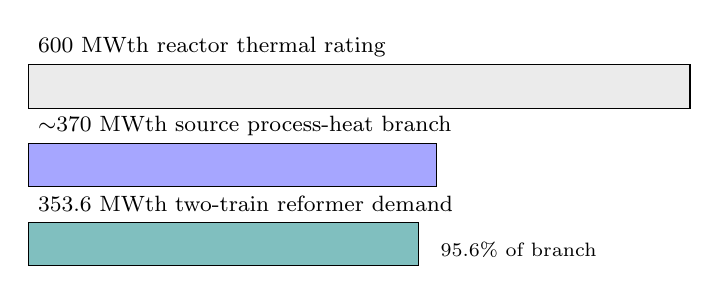
\begin{tikzpicture}[x=0.014cm,y=1cm,font=\footnotesize]
\draw[fill=gray!16] (0,1.8) rectangle (600,2.35);
\draw[fill=blue!35] (0,0.8) rectangle (370,1.35);
\draw[fill=teal!50] (0,-0.2) rectangle (353.6,0.35);
\node[anchor=west] at (0,2.58) {600 MWth reactor thermal rating};
\node[anchor=west] at (0,1.58) {$\sim$370 MWth source process-heat branch};
\node[anchor=west] at (0,0.58) {353.6 MWth two-train reformer demand};
\node[anchor=west] at (365,-0.0) {\scriptsize 95.6\% of branch};
\end{tikzpicture}
\caption{Nested thermal power scales, not a closed plant energy-flow diagram. The conditional 246.4 MWth difference between 600 and 353.6 MWth is not an established cooling, electricity or decay-heat duty.}
\label{fig:thermal-allocation-two-train}
\end{figure}}
\newcommand{\HydrogenScaleFigure}{%
\begin{figure}[htbp]\centering
\begin{tikzpicture}[>=Latex,font=\footnotesize,
 b/.style={draw=blue!65!black,fill=blue!5,rounded corners,align=center,text width=0.26\linewidth,minimum height=12mm}]
\node[b] (a) {Case-6 train A\\97,946 tH$_2$/y\\176.8 MWth};
\node[b,right=9mm of a] (b) {Case-6 train B\\97,946 tH$_2$/y\\176.8 MWth};
\node[b,below=12mm of $(a)!0.5!(b)$] (sum) {Project total\\195,892 tH$_2$/y\\353.6 MWth};
\draw[->,thick] (a.south)--(sum.north west);
\draw[->,thick] (b.south)--(sum.north east);
\end{tikzpicture}
\caption{Identical-train annual hydrogen scaling at assumed 85\% integrated availability. This is a project derivation from the INL per-train service, not a measured two-train facility.}
\label{fig:hydrogen-two-train}
\end{figure}}
\newcommand{\LifecycleFlowFigure}{%
\begin{figure}[htbp]\centering
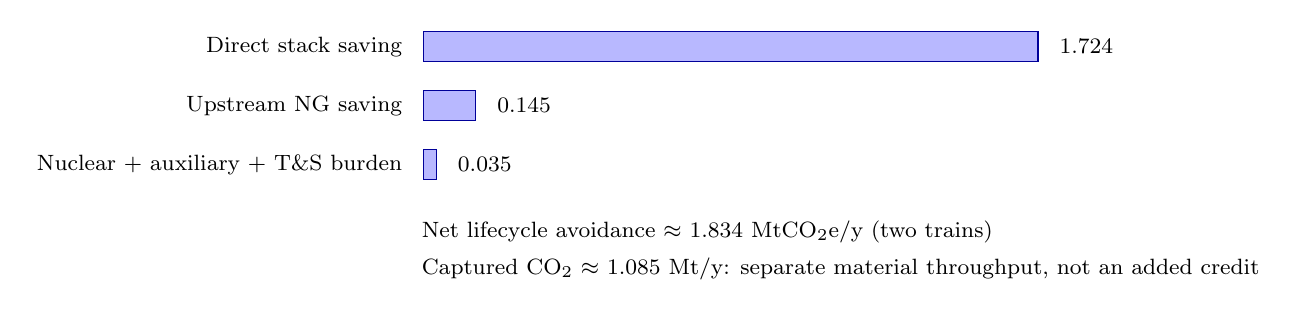
\begin{tikzpicture}[x=1cm,y=1cm,font=\footnotesize]
\foreach \y/\lab/\v/\len in {3/{Direct stack saving}/1.724/7.8,2.25/{Upstream NG saving}/0.145/0.66,1.5/{Nuclear + auxiliary + T\&S burden}/0.035/0.16}{
\node[anchor=east,align=right] at (0,\y) {\lab};
\draw[fill=blue!28,draw=blue!60!black] (0.15,\y-0.19) rectangle ({0.15+\len},\y+0.19);
\node[anchor=west] at ({0.3+\len},\y) {$\v$};
}
\node[anchor=west] at (0,0.65) {Net lifecycle avoidance $\approx$ 1.834 MtCO$_2$e/y (two trains)};
\node[anchor=west] at (0,0.18) {Captured CO$_2$ $\approx$ 1.085 Mt/y: separate material throughput, not an added credit};
\end{tikzpicture}
\caption{Two-train lifecycle components in MtCO$_2$e/y, rounded from the E2B per-train ledger. Direct and upstream savings are offset by added nuclear, auxiliary and transport/storage burdens; captured CO$_2$ is not double counted. Bar lengths are schematic and values control interpretation.}
\label{fig:lifecycle-two-train}
\end{figure}}
\newcommand{\EconomicsDecompositionFigure}{%
\begin{figure}[htbp]\centering
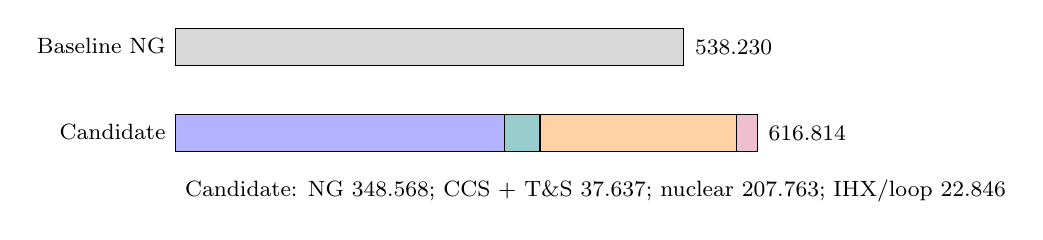
\begin{tikzpicture}[x=0.012cm,y=1cm,font=\footnotesize]
\node[anchor=east] at (0,2.2) {Baseline NG};
\draw[fill=gray!30] (0,1.95) rectangle (538.230,2.42);
\node[anchor=west] at (540,2.18) {538.230};
\node[anchor=east] at (0,1.1) {Candidate};
\draw[fill=blue!30] (0,0.85) rectangle (348.568,1.32);
\draw[fill=teal!40] (348.568,0.85) rectangle (386.205,1.32);
\draw[fill=orange!35] (386.205,0.85) rectangle (593.968,1.32);
\draw[fill=purple!25] (593.968,0.85) rectangle (616.814,1.32);
\node[anchor=west] at (618,1.08) {616.814};
\node[anchor=west] at (0,0.35) {Candidate: NG 348.568; CCS + T\&S 37.637; nuclear 207.763; IHX/loop 22.846};
\end{tikzpicture}
\caption{Represented mature 10-OAK annual cost ledger (S\$ million/y), not a complete project cost estimate. Difference $\sim$78.583 million S\$/y using unrounded Rust values; denominator 1.834278 MtCO$_2$e/y gives $\sim$S\$42.84/tCO$_2$e.}
\label{fig:two-train-economics-decomposition}
\end{figure}}
\newcommand{\MaturityComparisonFigure}{%
\begin{figure}[htbp]\centering
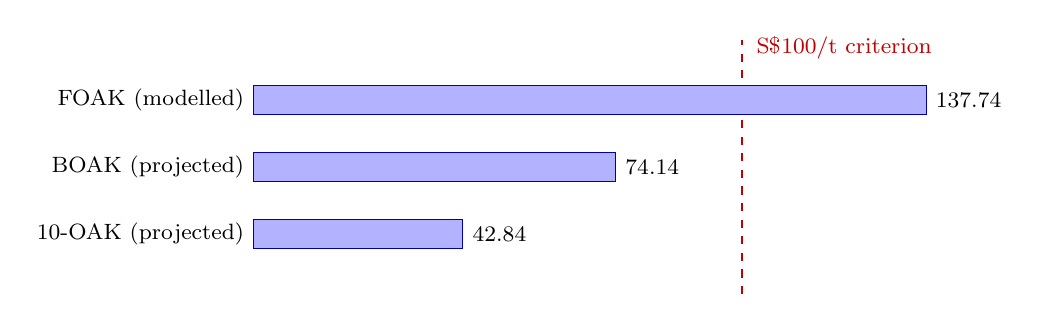
\begin{tikzpicture}[x=0.062cm,y=0.85cm,font=\footnotesize]
\draw[dashed,red!75!black,thick] (100,0.5)--(100,4.3);
\node[anchor=west,red!75!black] at (101,4.18) {S\$100/t criterion};
\foreach \y/\name/\value in {3.4/{FOAK (modelled)}/137.74,2.4/{BOAK (projected)}/74.14,1.4/{10-OAK (projected)}/42.84}{
\node[anchor=east] at (0,\y) {\name};
\draw[fill=blue!30,draw=blue!65!black] (0,\y-0.22) rectangle (\value,\y+0.22);
\node[anchor=west] at (\value,\y) {\value};
}
\end{tikzpicture}
\caption{Two-train modelled abatement cost (S\$/tCO$_2$e). FOAK fails the originating S\$100/t screen; future BOAK and 10-OAK numerical passes rely on projected cost learning, not observed construction.}
\label{fig:two-train-maturity}
\end{figure}}
\newcommand{\UncertaintyDriversFigure}{%
\begin{figure}[htbp]\centering
\begin{tikzpicture}[>=Latex,font=\footnotesize,
 b/.style={draw=blue!60!black,rounded corners,fill=blue!4,text width=0.24\linewidth,align=center,minimum height=12mm}]
\node[b] (cost) {Annual represented cost\\Construction learning, site, licensing, IHX, CCS};
\node[b,right=8mm of cost] (avoid) {Avoided lifecycle emissions\\Availability, NG upstream, capture, T\&S};
\node[b,below=12mm of $(cost)!0.5!(avoid)$] (ratio) {Abatement cost\\$\Delta C_y/A_y$};
\draw[->,thick] (cost.south)--(ratio.north west);
\draw[->,thick] (avoid.south)--(ratio.north east);
\end{tikzpicture}
\caption{Uncertainty-driver map, not a probabilistic tornado chart. No project-specific distributions or two-train sensitivity ranges are available; historical one-train numerical sensitivities remain in Appendix~\ref{app:historical-sensitivity}.}
\label{fig:two-train-uncertainty}
\end{figure}}
